\documentclass[12pt]{article}
\usepackage{amsmath,amssymb, fixltx2e, graphicx, tikz, color, enumerate,blindtext, epstopdf, geometry}
\newcommand\lr{\left \langle}
\newcommand\rr{\right \rangle}
\newcommand\tbf[1]{\textbf{1}}
%\DeclareGraphicsExtensions{.eps}
%\DeclareGraphicsExtensions{.tex}
\title{\textbf{Transient behaviour of a Lazy Random Walker in One Dimension}}
\author{Sunip Kumar Mukherjee \\ Muktish Acharyya \\ Department of Physics, Presidency University, \\ 86/1 College Street, Kolkata-700073, INDIA \\ Email: sunipkmukherjee@gmail.com, muktish.physics@presiuniv.ac.in}
\begin{document}
\maketitle
\textbf{ABSTRACT: }The motion of a lazy random walker is studied in one dimension. With a more physical definition of laziness, the diffusion of the walker is observed. The first return probability is also numerically calculated for the walker, for various laziness ``levels'', and a comparison is made for various laziness levels, including a normal random walker. A relation of the kind $\left \langle d^2 \right \rangle = a\times \left \langle t_{fr} \right \rangle ^b$ is established, with the value of the exponent exactly 3, for all laziness levels in the transient analysis of the first return probability for the random walker. It is also established that the first return probability in the transient region is always higher for higher value of laziness, for a given time limit to the random walker, and ultimately the probability converges (asymptotically) to 1. \\

\vspace{1.2 cm}
\textbf{Keywords: Lazy random walk, first return probability, scaling}
\newpage
\begin{enumerate}[I.]
  \item \textbf{INTRODUCTION: } \\

    \blindtext[2]
    \item \textbf{MODEL and RESULTS: } \\

Mathematically, a lazy random walk is described where the walker has 50\% probability of moving from his current position, and in one dimension has equal probability of moving in either direction. In this paper, a more physical approach is taken towards laziness. Here, laziness is defined as a continuous variable ranging from 0 to 1, where 0 laziness parameter signifies an ordinary random walk, and laziness parameter 1 signifies the case where the walker does not move at all, being completely lazy. In practise, if $P_{lazy}$ is the laziness parameter, the walker has $P_{lazy}\times 100 \%$ chance of \emph{not} moving from that position. Once the walker decides to move, he has equal probability of moving either right or left. The diffusion of such a walker is first investigated, over a large number of samples, i.e. by releasing the random walker many times. The random walker is allowed to move for a certain amount of time, and the final position of the walker is noted after the allowed time has elapsed, and the distribution of the final position is obtained for the given sample size. For a large enough sample, the distribution is Gaussian, and in the asymptotic limit, it can be established theoretically that the distribution is indeed Gaussian. For a normal random walker, this result is already established. For a mathematical random walker, this result can also be simulated. For the definition of a lazy walker given above, the same behaviour is observed, as the reader can verify from the accompanying figures. As one intuitively expects, the ``lazy walker'', given the same amount of time should not travel further than the normal walker, and ``lazier'' walker will travel even less. So, for the same amount of allowed time, the normal walker will move around the furthest and have a rather wide distribution of displacement, and the width of the distribution will diminish with increasing laziness. But for the same laziness parameter, the walker is again expected to diffuse, i.e. to travel further, with more allowed time. This is also established in the accompanying figures. Mostly a lazy random walker behaves like a normal random walker. The ``activity parameter'' of a lazy random walker is defined simply by $P_{act}=1-P_{lazy}$. A normal random walker is thus ``fully active'' and an absolutely lazy random walker ($P_{lazy}=1$) is completely inactive. In this paper, the term step is equivalent to unit time, and a step size limit determines how long a walker is allowed to walk. With a given step size limit, i.e. finite amount of time and non zero activity parameter, an ensemble of identical random walkers will end up to be at different positions after walking for the alloted ``time'' or step size limit, and we can obtain a distribution of the probability for the walker to be at some distance from the origin, and regardless of the newly introduced laziness parameter the distribution is Gaussian. This can be observed in Figure \ref{fig:distribution}, and Figure \ref{fig:dist_st}. These observation prompted the assumption of a scaling behaviour involving both the ``step size limit ($T_{max}$)'', as the distribution width clearly depends on it, as well as the ``activity parameter ($P_{act}$)'' and equivalently the ``laziness parameter''. By $P_r$ the probability of finding a random walker at a distance $r$ from the origin is denoted. A scaling like $aP_r T_{max}^\alpha P_{act}^\beta = \exp(-bT_{max}^\gamma P_{act}^\delta r^2)$ is assumed, and the various distribution curves (all denoted by the different symbols for different sets of $T_{max}$ and $P_{act}$) collapses to $\exp(-x^2)$, as is observed in Figure~\ref{fig:dist_sc} with $a=1/4$, $b=0.5$, $\alpha=\beta=-0.5$, and $\gamma=\delta=-1$. It may be mentioned here that the statistics is based on $N_s=10^7$ different random samples. That the exponents $\alpha$, $\beta$ and $\gamma$, $\delta$ are the same is expected, as the activity parameter simply modulates the step size limit for a statistical ensemble, i.e. a lazy walker statistically is able to move for only $P_{act}\cdot T_{max}$ amount of time.  \\ \newline The next interesting property of such walkers that has been investigated, is the first return probability. After the random walker sets out, in one dimension, given infinite time, a normal walker returns with a certainty to the place where it started from. Which implies that the return probability is 1. But, given finite amount of time, the probability is not exactly 1, but is somewhat less, and this number increases with the amount of time, asymptotically, to one, as Figure~\ref{fig:frp_var} clearly shows. %But the more important feature is rather non intuitive, which reveals itself upon the incorporation of the laziness parameter. Since the laziness increases the chance that the walker is not moving most of the time, we should expect that the walker will not be able to return as many times an active ($P_{lazy}=0$) walker does, i.e. the return probability $P_{ret}$ will be less for a lazy walker, than it is for an active walker. However, simulations with sample size of 100000 and also 100000000 (the sample size indicates how many times a walker was released from the origin for a certain amount of time with a certain laziness parameter), and the plots generated from the data (refer to Figure~\ref{fig:frp_var}) indicates that for a given amount of time, the lazier the walker, the higher is the return probability. The accompanying plots are given for sample size of 100000, with the time (step size, where the unit of time is designated by each step) ranging from 10 to 100000, we see that the lazier walker always has the higher probability of returning. Due to constraints on the computational capabilities, not much work has been done on the case of very very large samples (100000000 samples). But for 10 timesteps, results on simulating the walk with laziness parameter ($P_{lazy}$) as 0 (normal random walker) and 0.8 (very lazy random walker) do indicate that the lazier walker has higher return probability (0.753 and 0.867 respectively). \\
%\newline This counter intuitive result is somewhat expected, given the lazy walker, by the virtue of laziness, never wanders too far from the starting point. Hence, he can very easily return to the starting point, whereas a normal walker may wander very far in the same span of time, as the active walker moves all the time. This claim is supported by the following observation: For a given time limit (step size), and for the various laziness levels (0, 0.2 $\cdots$, 0.8),  we calculate the mean squared distance travelled by the walker in case he returns, and the average time taken by the walker to return. Obviously, with increasing laziness, for the same amount of allowed time, the walker is found to move less further, i.e. the mean squared distance turns out to be less. Interestingly, the average time of return is also less with laziness. For a given step size, if the mean squared distance (for the walks where there was a return) is plotted with respect to the average time for first return, we obtain a nice power law of the form $\left \langle d^2 \right \rangle = a \times \left \langle t \right \rangle ^3$. Interestingly, the coefficient $a$ is the same for all the step sizes, from as low as 10 to as high as 1000000, and this power law is maintained throughout, with different ``bands'' formed by points corresponding to different laziness parameters given the same amount of time. The reader, in this context, is reminded of the \emph{Child-Langmuir's law of current flow due to space charge} in a thermal diode, for example, where a law of the similar form $I=a\times V^{\frac{3}{2}}$ holds, where $I$ is the current due to space charge, and $V$ is the potential difference from the anode to the cathode. However, no effort is made in this paper to relate Child-Langmuir's law to the power law demonstrated here.
In fact, as \emph{Poyla} showed in his papers, the convergence is as $1-\frac{1}{\sqrt{2t}}$, a result which is re-established in the accompanying figure. Figure~\ref{fig:frp_var} contains the plot of $P_{fr}$ \emph{vs.} $t_{max}$, for various laziness parameters, and all the curves show the same behaviour as of the normal random walker, the only difference being that $P_{fr}$ is less for the same $t_{max}$ with increasing laziness. Which is expected, as with increasing laziness parameter, the walker has less chance of moving about. So, from Figure~\ref{fig:frp_var}, it is expected that the $P_{fr}$ \emph{vs.} $t_{max}$ plots for various laziness parameters can be scaled to a single curve. Since $P_{act}\times t_{max}$ gives (probalistically) the time utilized by the lazy walker, this form of scaling is expected, and the requisite scaling produces the data collapse described in Figure~\ref{fig:frp_scale}, and all the points collapse to the curve $1-\frac{1}{\sqrt{1.65\times t_{max}}}$. As a cross check, $P_{fr}=0.45$ for $t_{max}=2$ from this curve, which is close to the actual probability, 0.5. This discrepancy is of course an inevitable consequence of having a finite size of the ensemble in numerical simulations.
\newline
Next, the two quantities $\lr t_{fr} \rr$ and $\lr d_{max}^2 \rr$ are studied. $\lr t_{fr} \rr$ is defined as the time taken for a walker (either lazy or non lazy) to return to the origin, within a given limit $t_{max}$. It must be understood that, for \tbf{returning}, the walker must be displaced from the origin at first. This is unimportant for an ordinary random walker, but for a lazy random walker it may be the case that the walker never moves withing the given time limit. Such cases are of course not treated as a successful return to the origin, as the walker had not moved out in the first place. In the cases the walker \emph{does} move out of the starting point, the total time that the walker takes to get back to the origin after the walker is allowed to move is counted, i.e. say the walker does not move at the first few steps, but does move out of the origin and returns. Then the first few steps are \tbf{not} discarded. $d_{max}$ is the maximum distance the walker moves away from the origin \tbf{before returning to the origin}. $d_{max}^2$ is averaged over an ensemble of random walkers. Figure~\ref{fig:pow_law} contains the plot of $\lr d_{max}^2 \rr$ vs $\lr t_{fr} \rr$, for laziness parameters ranging from $0$ to $0.9$, and different values of $t_{max}$. It is evident, that the points for different laziness parameters but with same $t_{max}$ group up, and for these point groups, a $P_{act}^{-1}$ behaviour is observed. However, $\lr d_{max}^{2} \rr$ vs $ \lr t_{fr} \rr$ shows a behaviour like $\lr d_{max}^{2} \rr = A\times P_{act} \times \lr t_{fr} \rr$. Again, we observe the similar scaling behavior, as plotted in Figure~\ref{fig:pow_law2}.

\end{enumerate}
\newpage

\begin{figure}
\centering
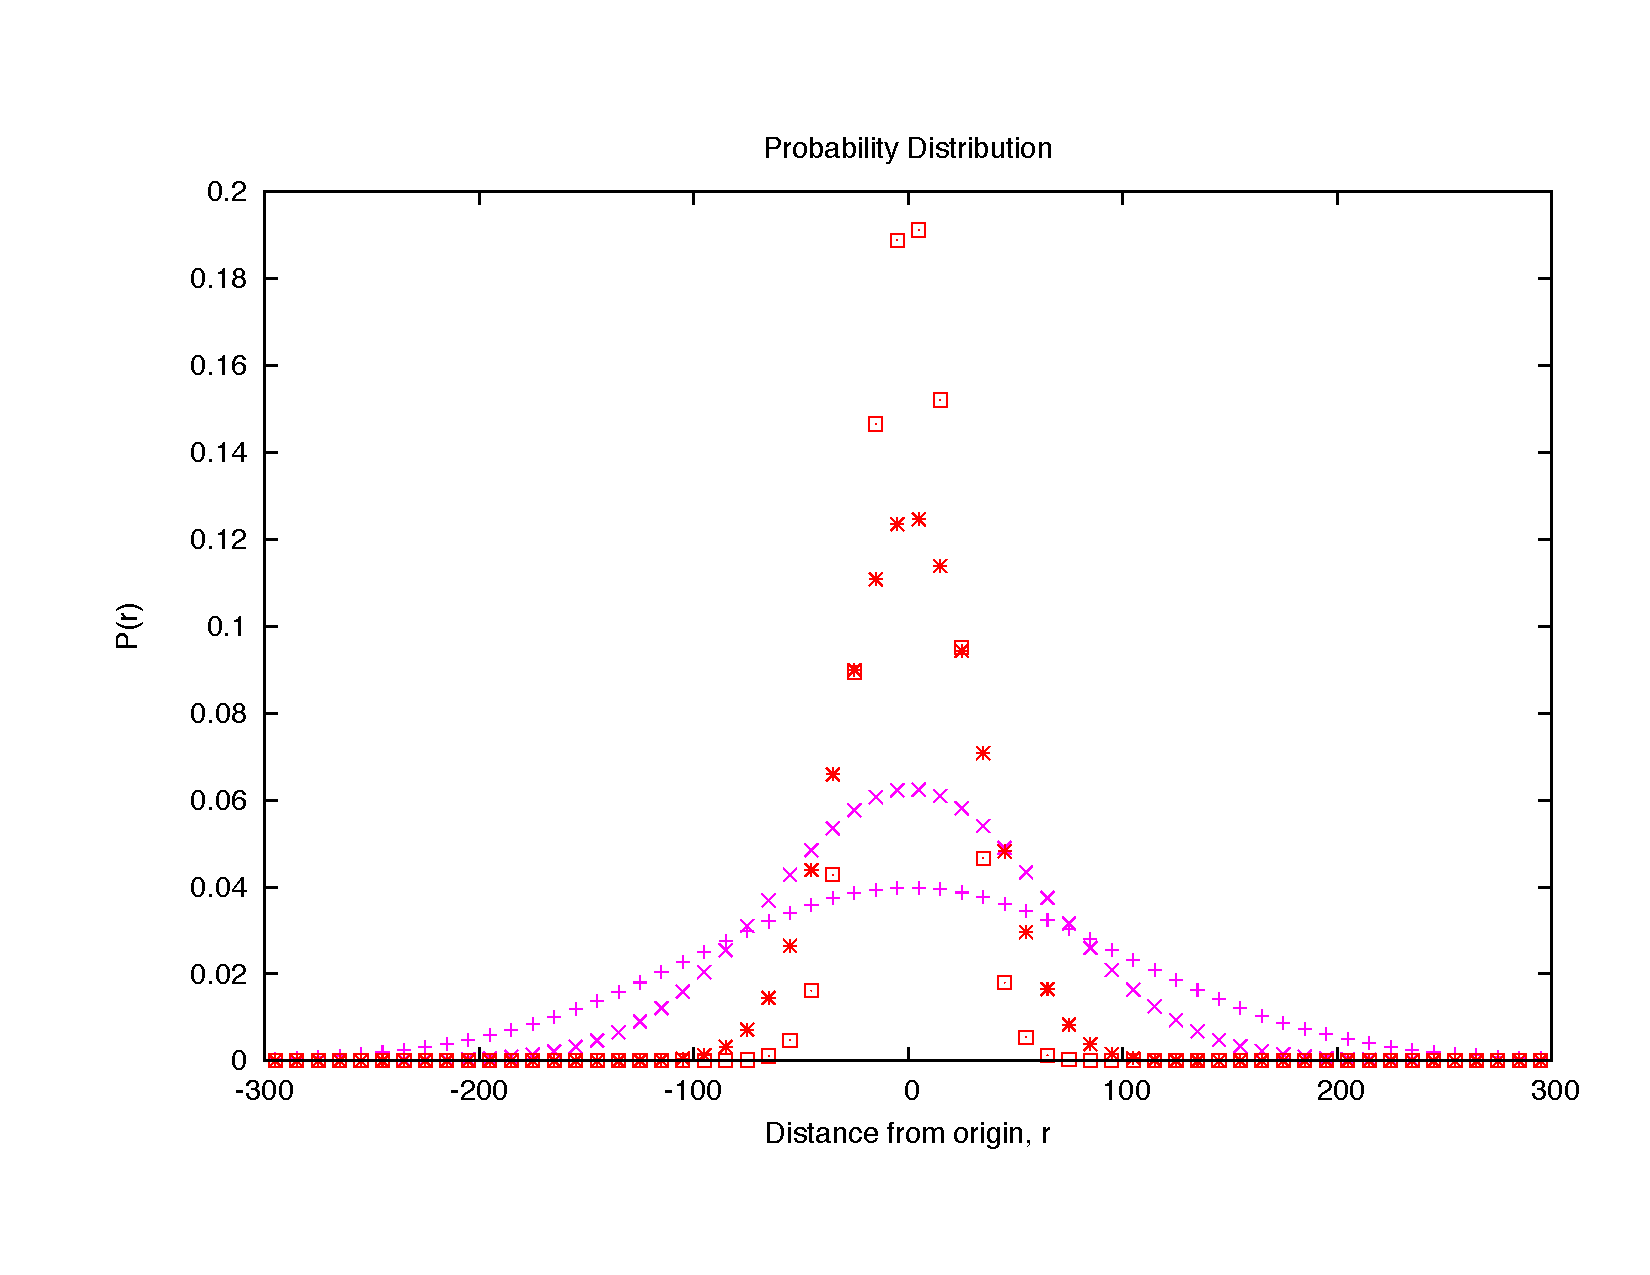
\includegraphics[width=\textwidth]{distribution.pdf}
\caption{$P_r$ vs. $r$ plot for 1000 and 10000 step size limits, and laziness 0 and 0.6. ``+'' denotes random walk with 10000 steps, 0 laziness. ``$\times$'' denotes the same with 10000 steps, 0.6 laziness, ``$\ast$'' denotes 1000 stepsize, 0.0 laziness and ``$\Box$'' denotes 1000 stepsize and 0.6 laziness.}
\label{fig:distribution}
\end{figure}

\newpage
\begin{figure}
\centering
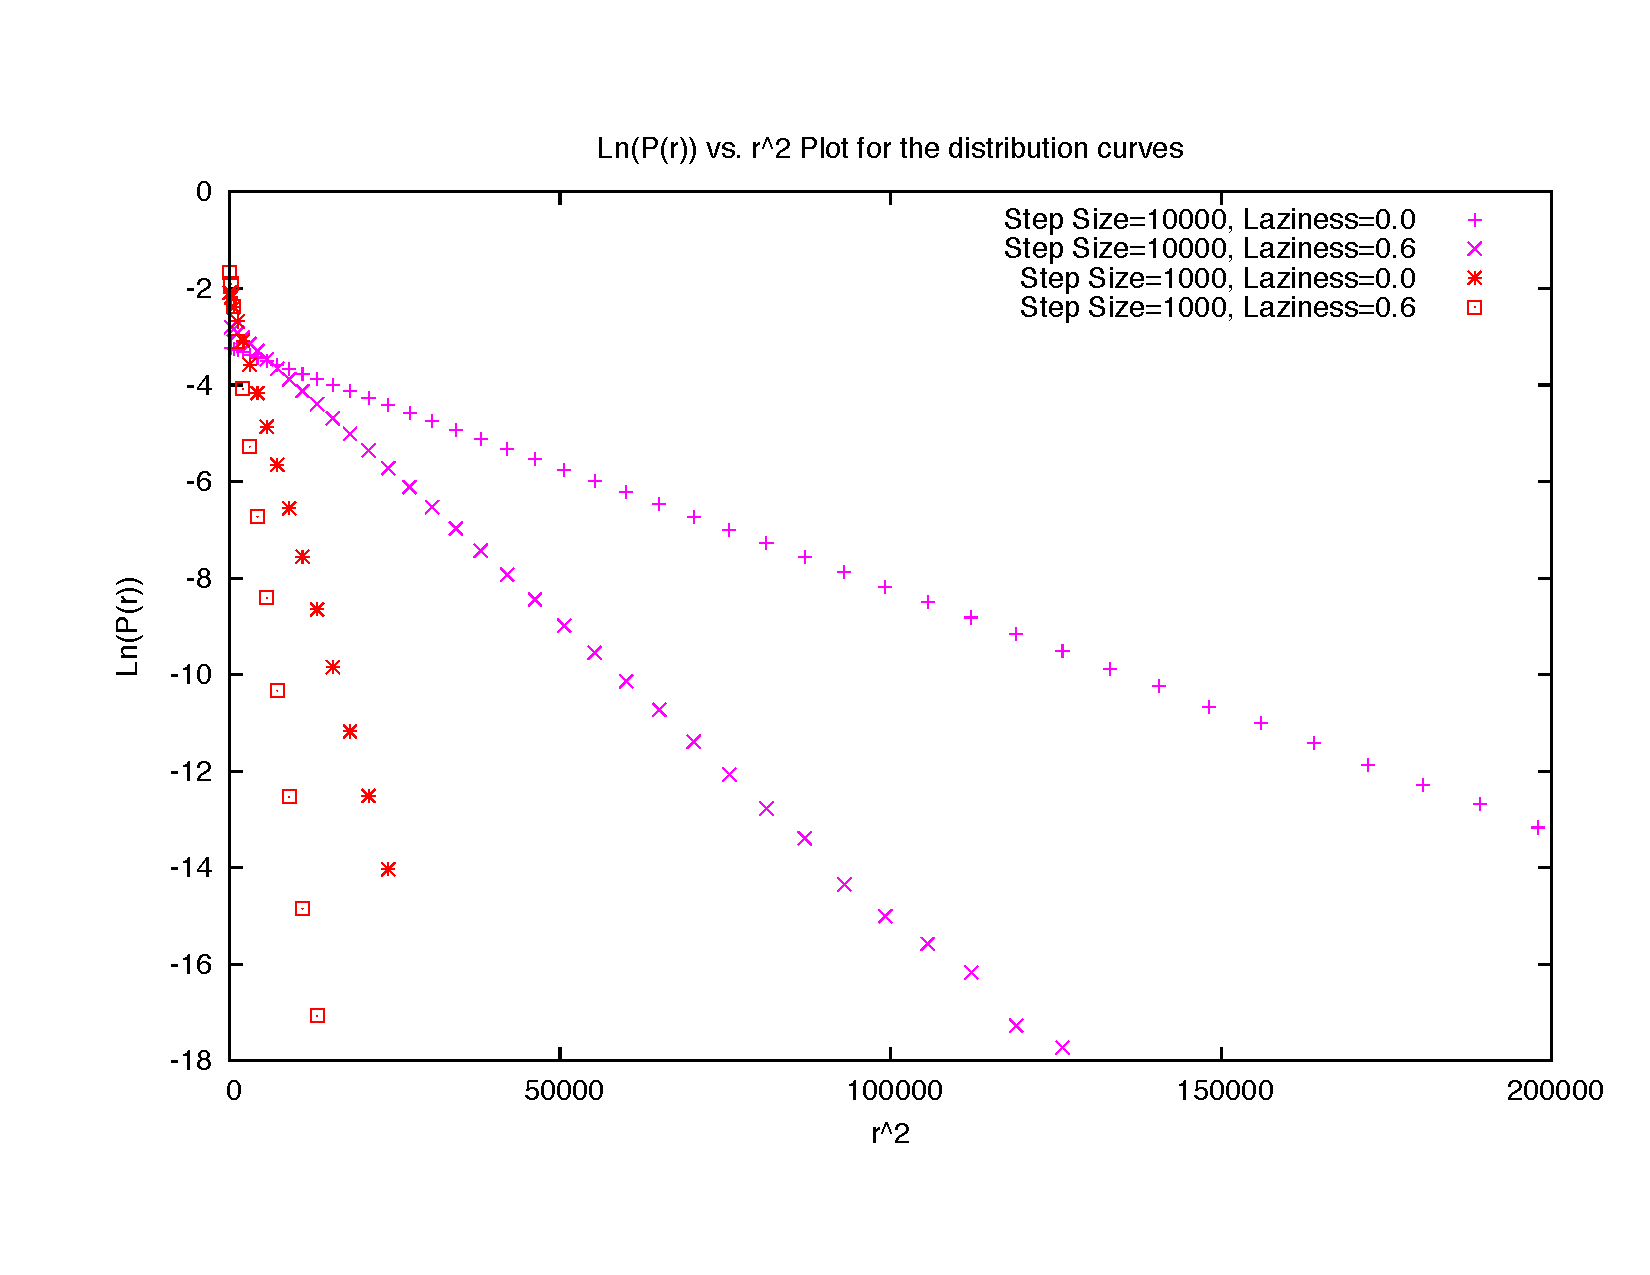
\includegraphics[width=\textwidth]{dist_st.pdf}
\caption{$P_r$ vs. $r$ plot for 1000 and 10000 step size limits, and laziness 0 and 0.6. ``+'' denotes random walk with 10000 steps, 0 laziness. ``$\times$'' denotes the same with 10000 steps, 0.6 laziness, ``$\ast$'' denotes 1000 stepsize, 0.0 laziness and ``$\Box$'' denotes 1000 stepsize and 0.6 laziness.}
\label{fig:dist_st}
\end{figure}

\newpage
\begin{figure}
\centering
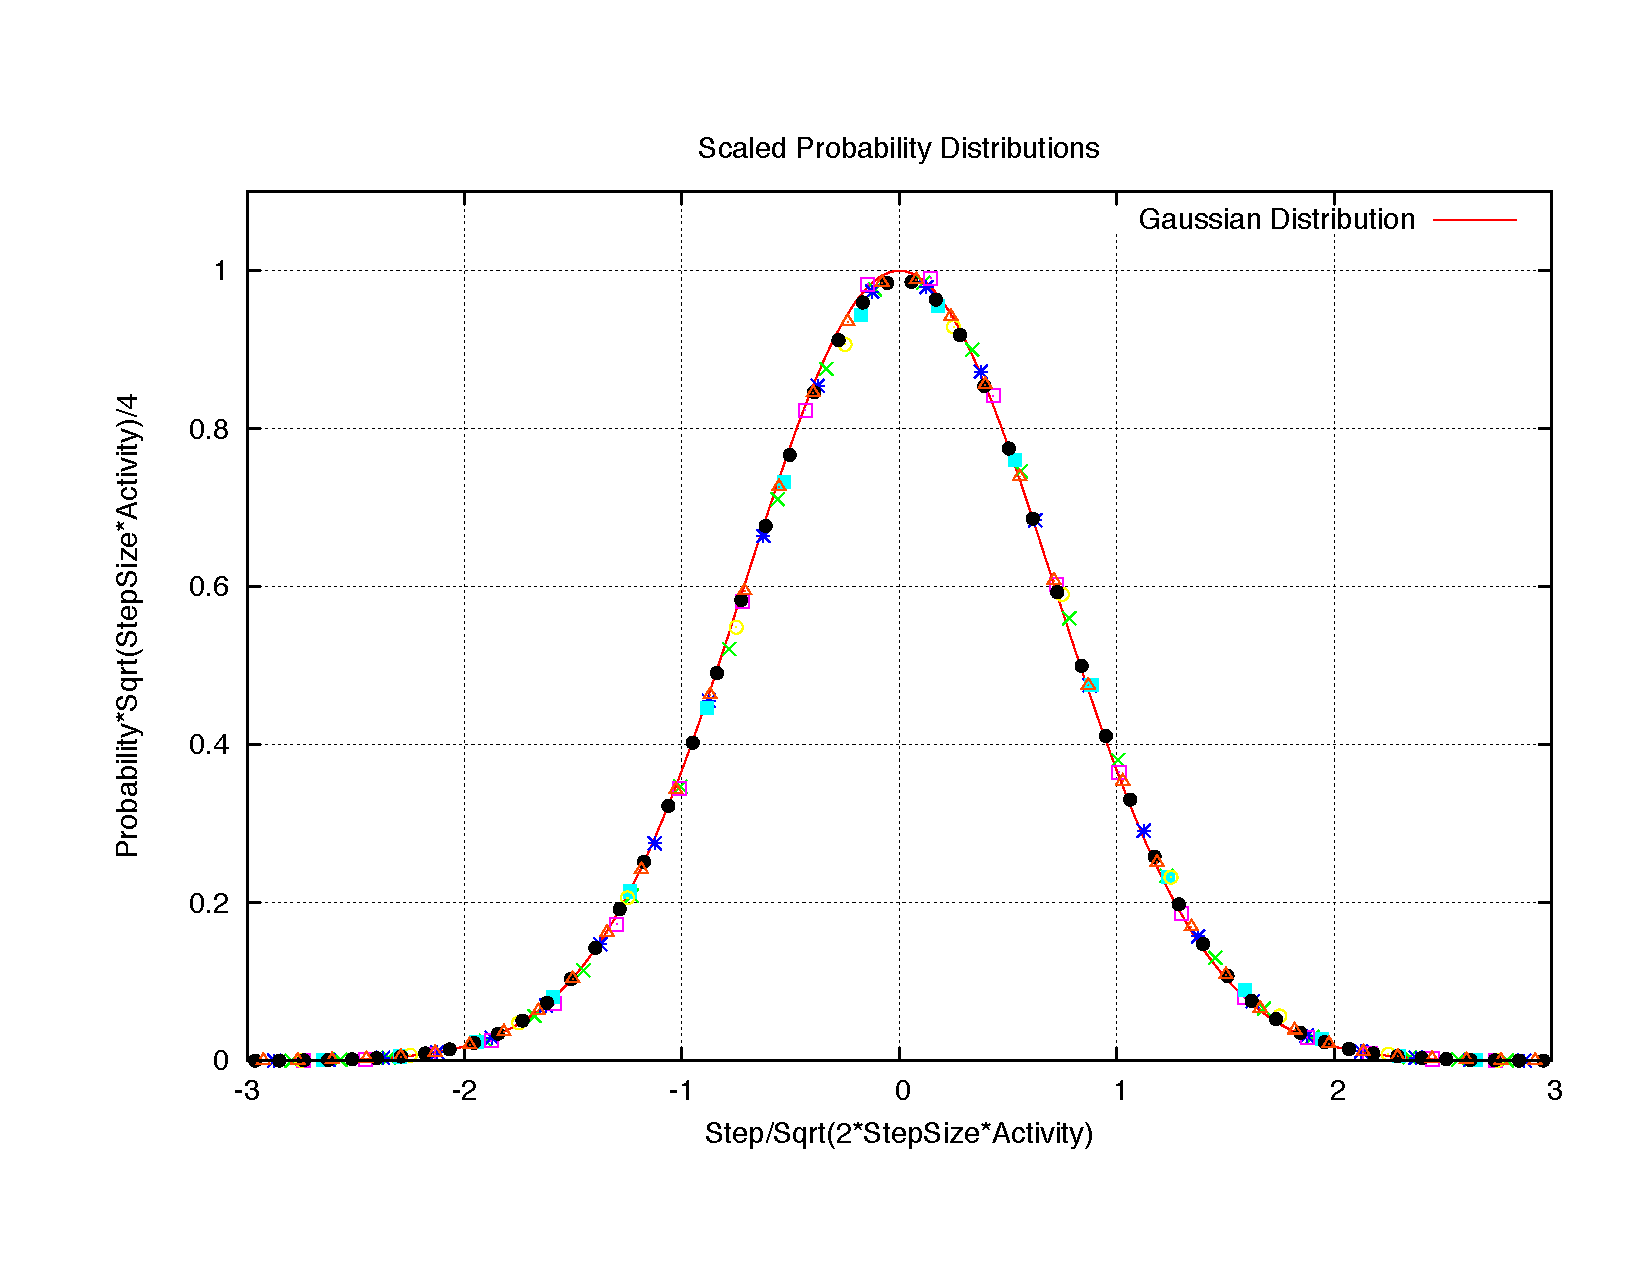
\includegraphics[width=\textwidth]{dist_sc.pdf}
\caption{$P_r \cdot \sqrt{P_{act} \cdot T_{max}}/4$ vs. $\sqrt{2\cdot P_{act} \cdot T_{max}}r$ plot for all step size limit ($T_{max}$) and all laziness parameters ($P_{lazy}$), and the scaling is apparent from the data collapse.}
\label{fig:dist_sc}
\end{figure}

\newpage
%FRP variation plot
\begin{figure}
\centering
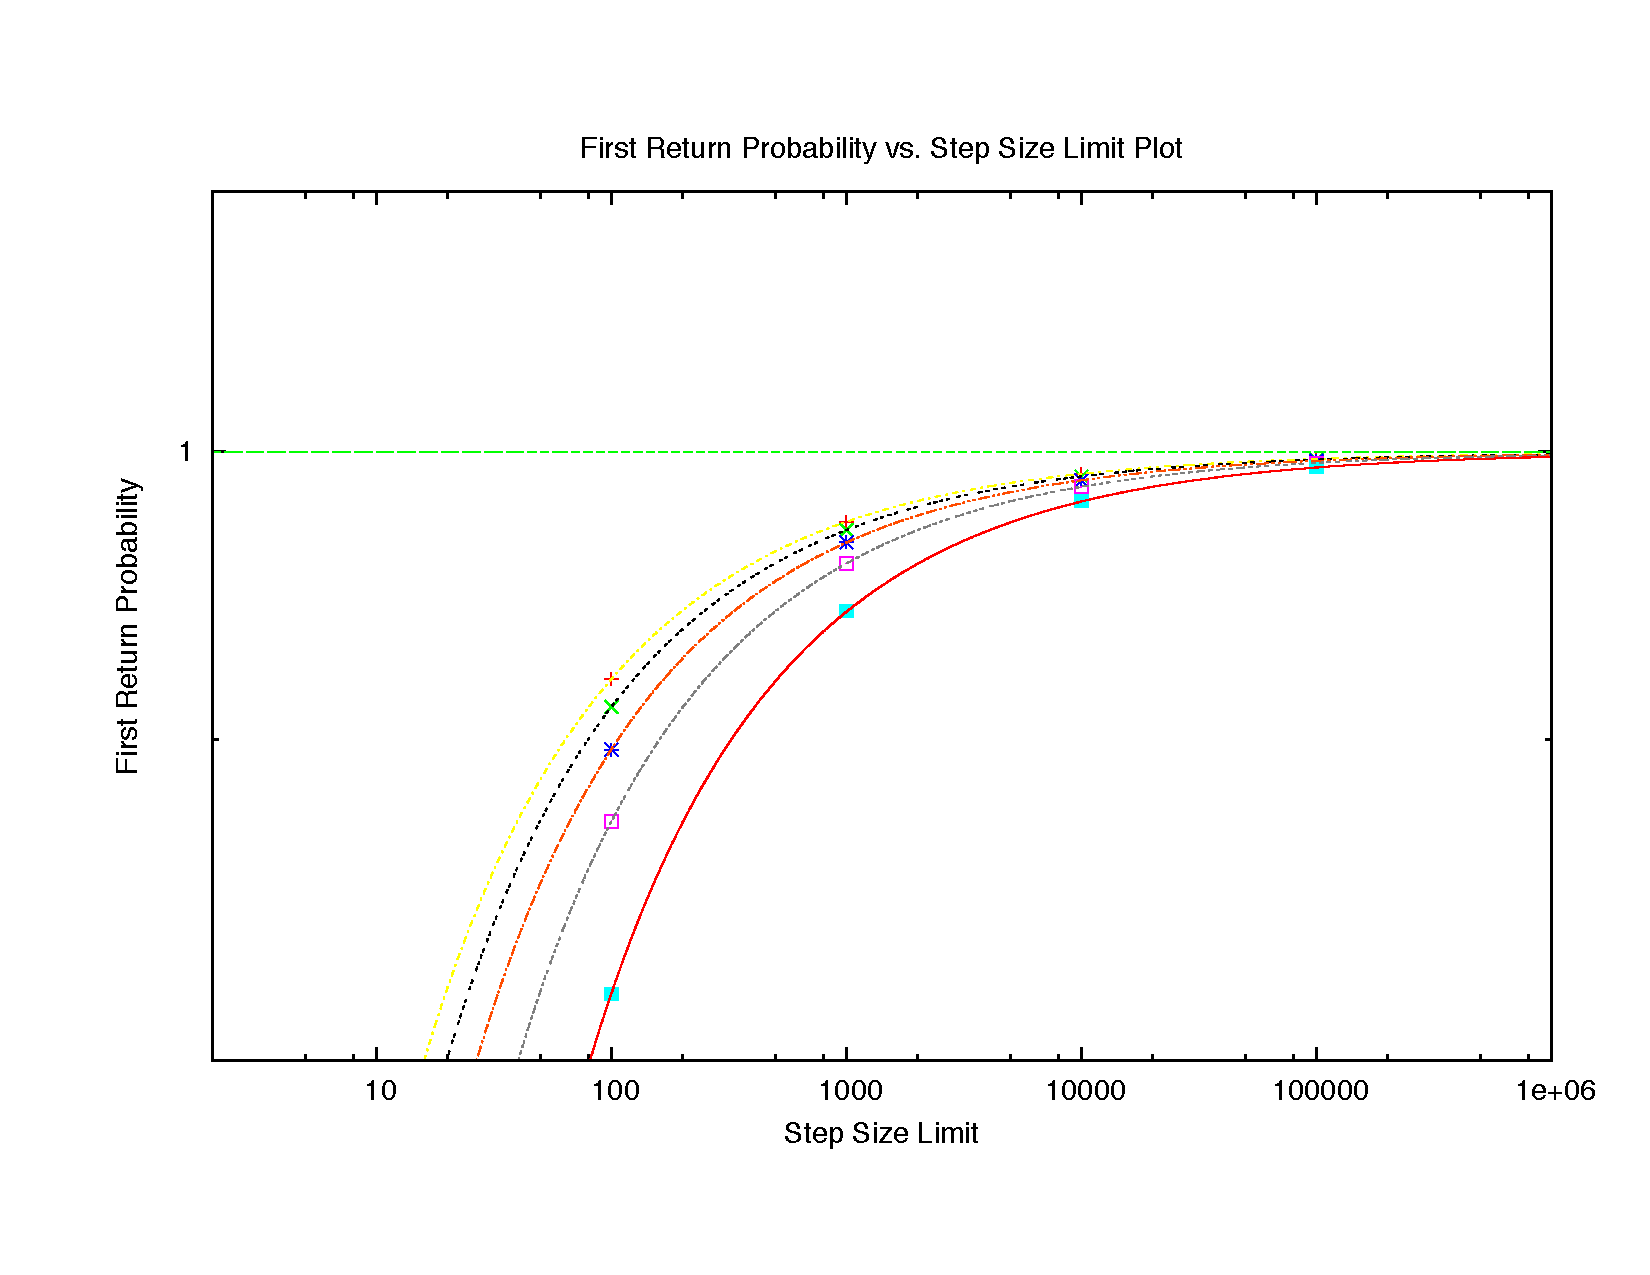
\includegraphics[width=\textwidth]{unscaled_frp.pdf}
\caption{$P_{FR}$ vs. $t_{max}$ plot with laziness from 0 to 0.8. ``+'' denotes random walk 0 laziness. ``$\times$'' denotes the same 0.2 laziness, ``$\ast$'' denotes 0.4 laziness, ``$\Box$'' denotes0.6  laziness, and $\blacksquare$ denotes 0.8 laziness.}
\label{fig:frp_var}
\end{figure}

\newpage
%FRP variation plot
\begin{figure}
\centering
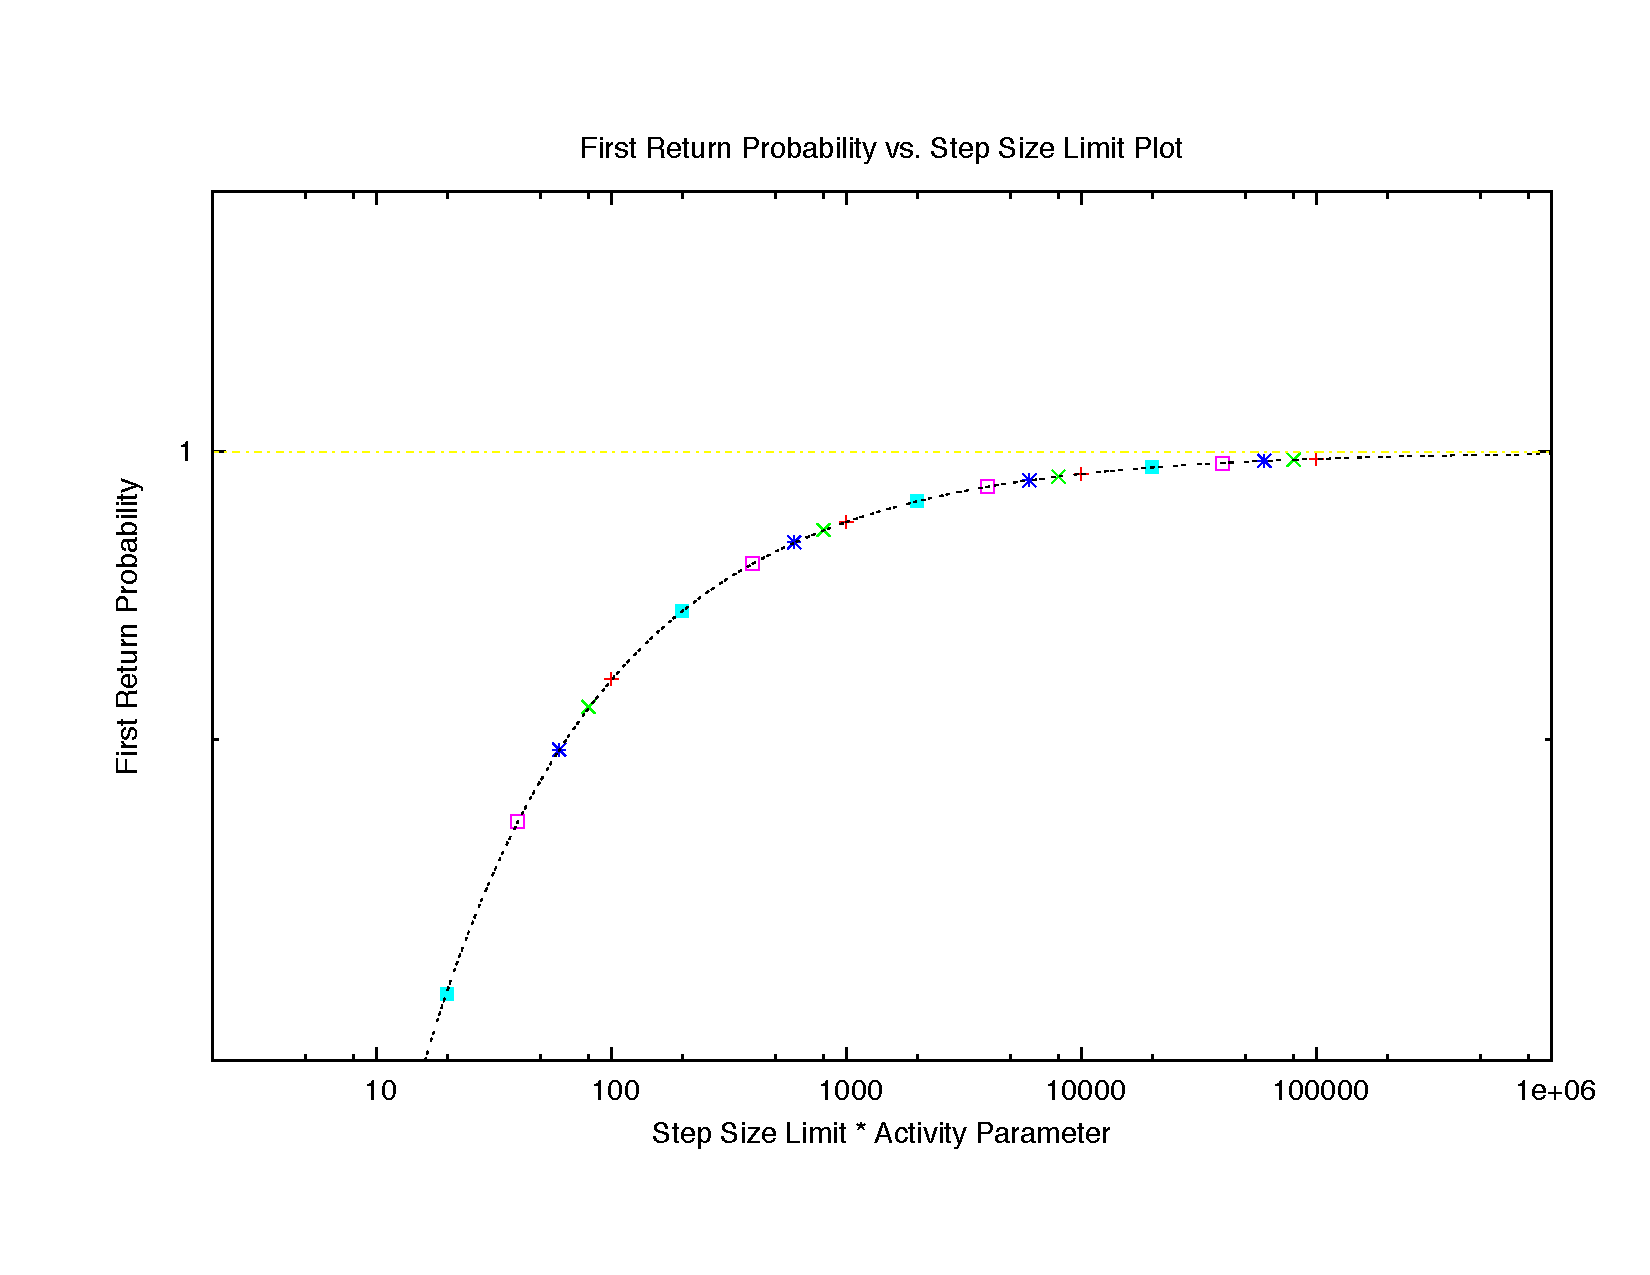
\includegraphics[width=\textwidth]{scaled_frp.pdf}
\caption{$P_{FR}$ vs. $(a/P_{act})t_{max}$ plot for laziness from 0 to 0.8. ``+'' denotes random walk 0 laziness. ``$\times$'' denotes the same 0.2 laziness, ``$\ast$'' denotes 0.4 laziness, ``$\Box$'' denotes0.6  laziness, and $\blacksquare$ denotes 0.8 laziness.}
\label{fig:frp_scale}
\end{figure}


\newpage
%unscaled stline plot
\begin{figure}
\centering
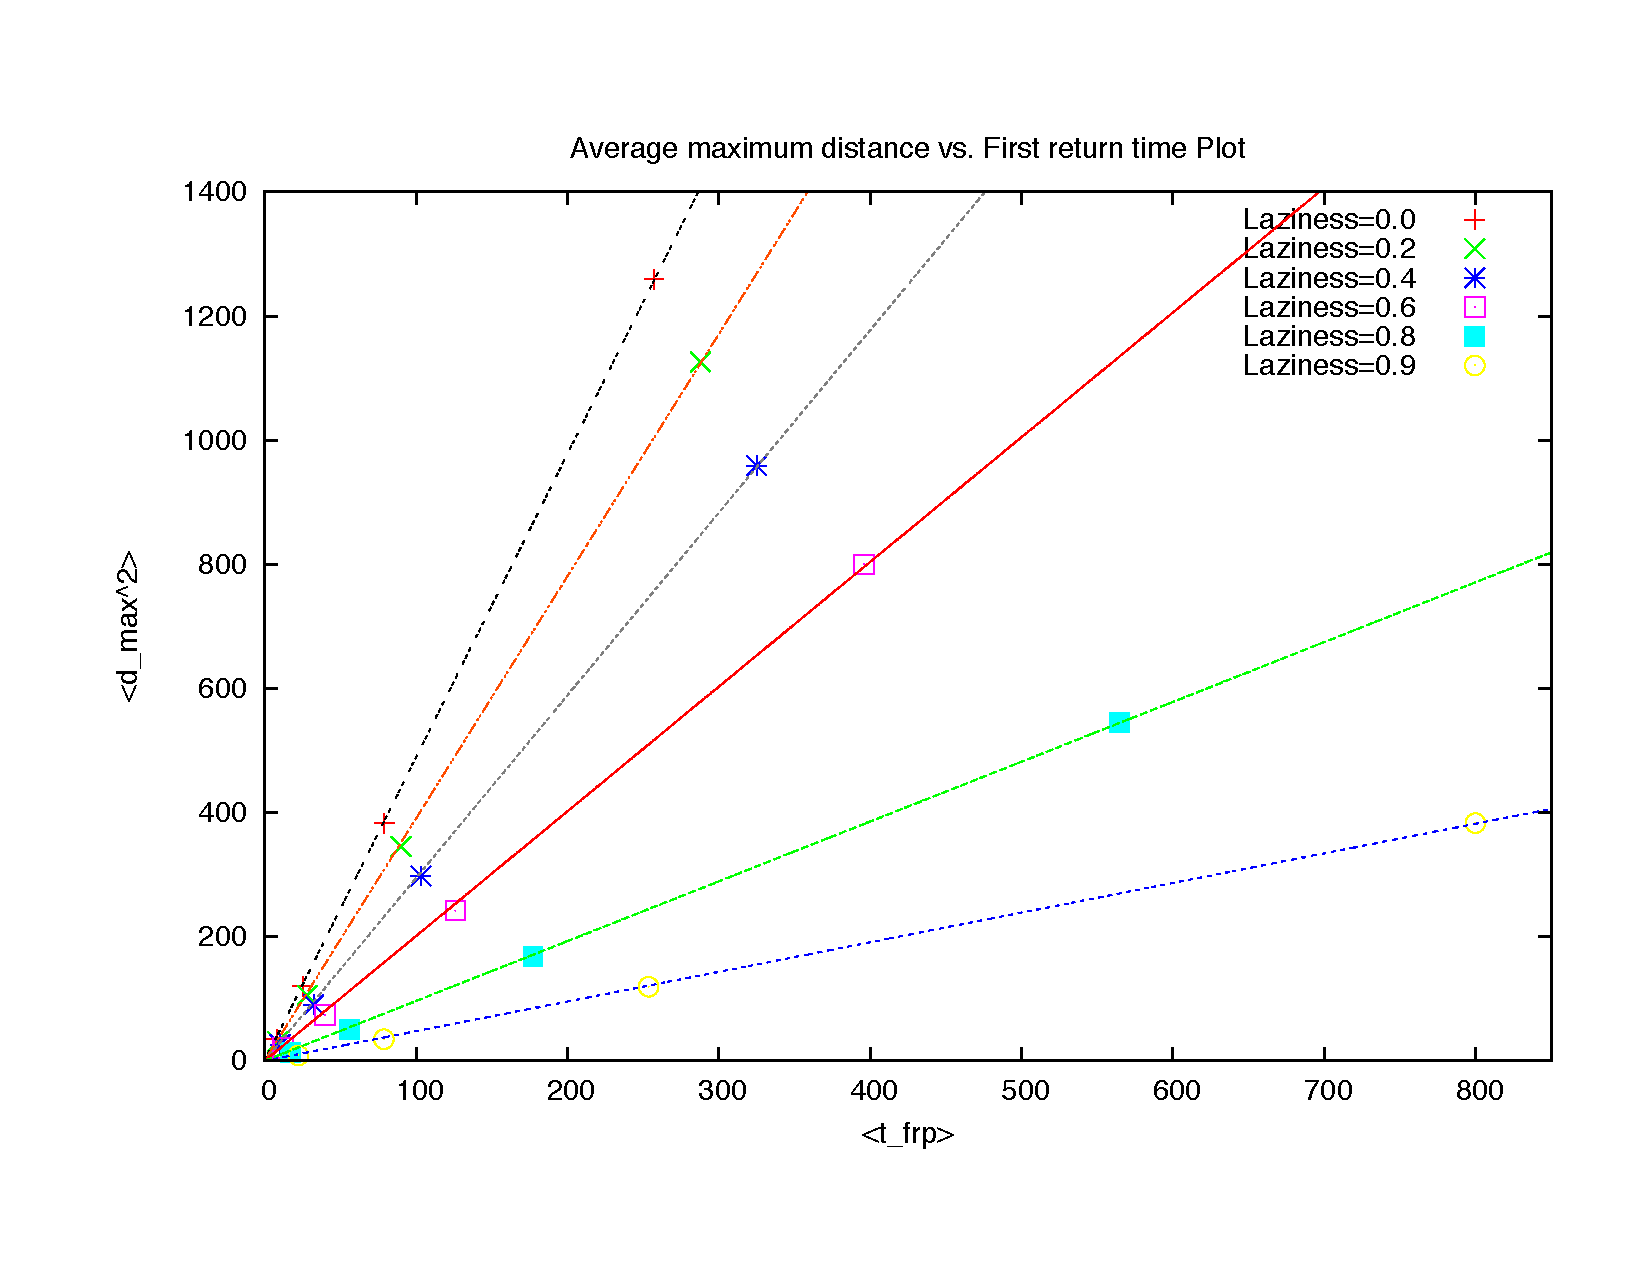
\includegraphics[width=\textwidth]{tfrp_unscaled.pdf}
\caption{$\langle d_{{max}} \rangle ^2$ vs. $\langle t_{FR} \rangle$ plot for laziness from 0 to 0.9, and $t_{max}$ ranging from 100 to 100000 in a geometric progression. Each $t_{max}$ has a group of points, and in each group the points are arranged in decreasing order of laziness.}
\label{fig:pow_law}
\end{figure}

\newpage
%scaled single line plot
\begin{figure}
\centering
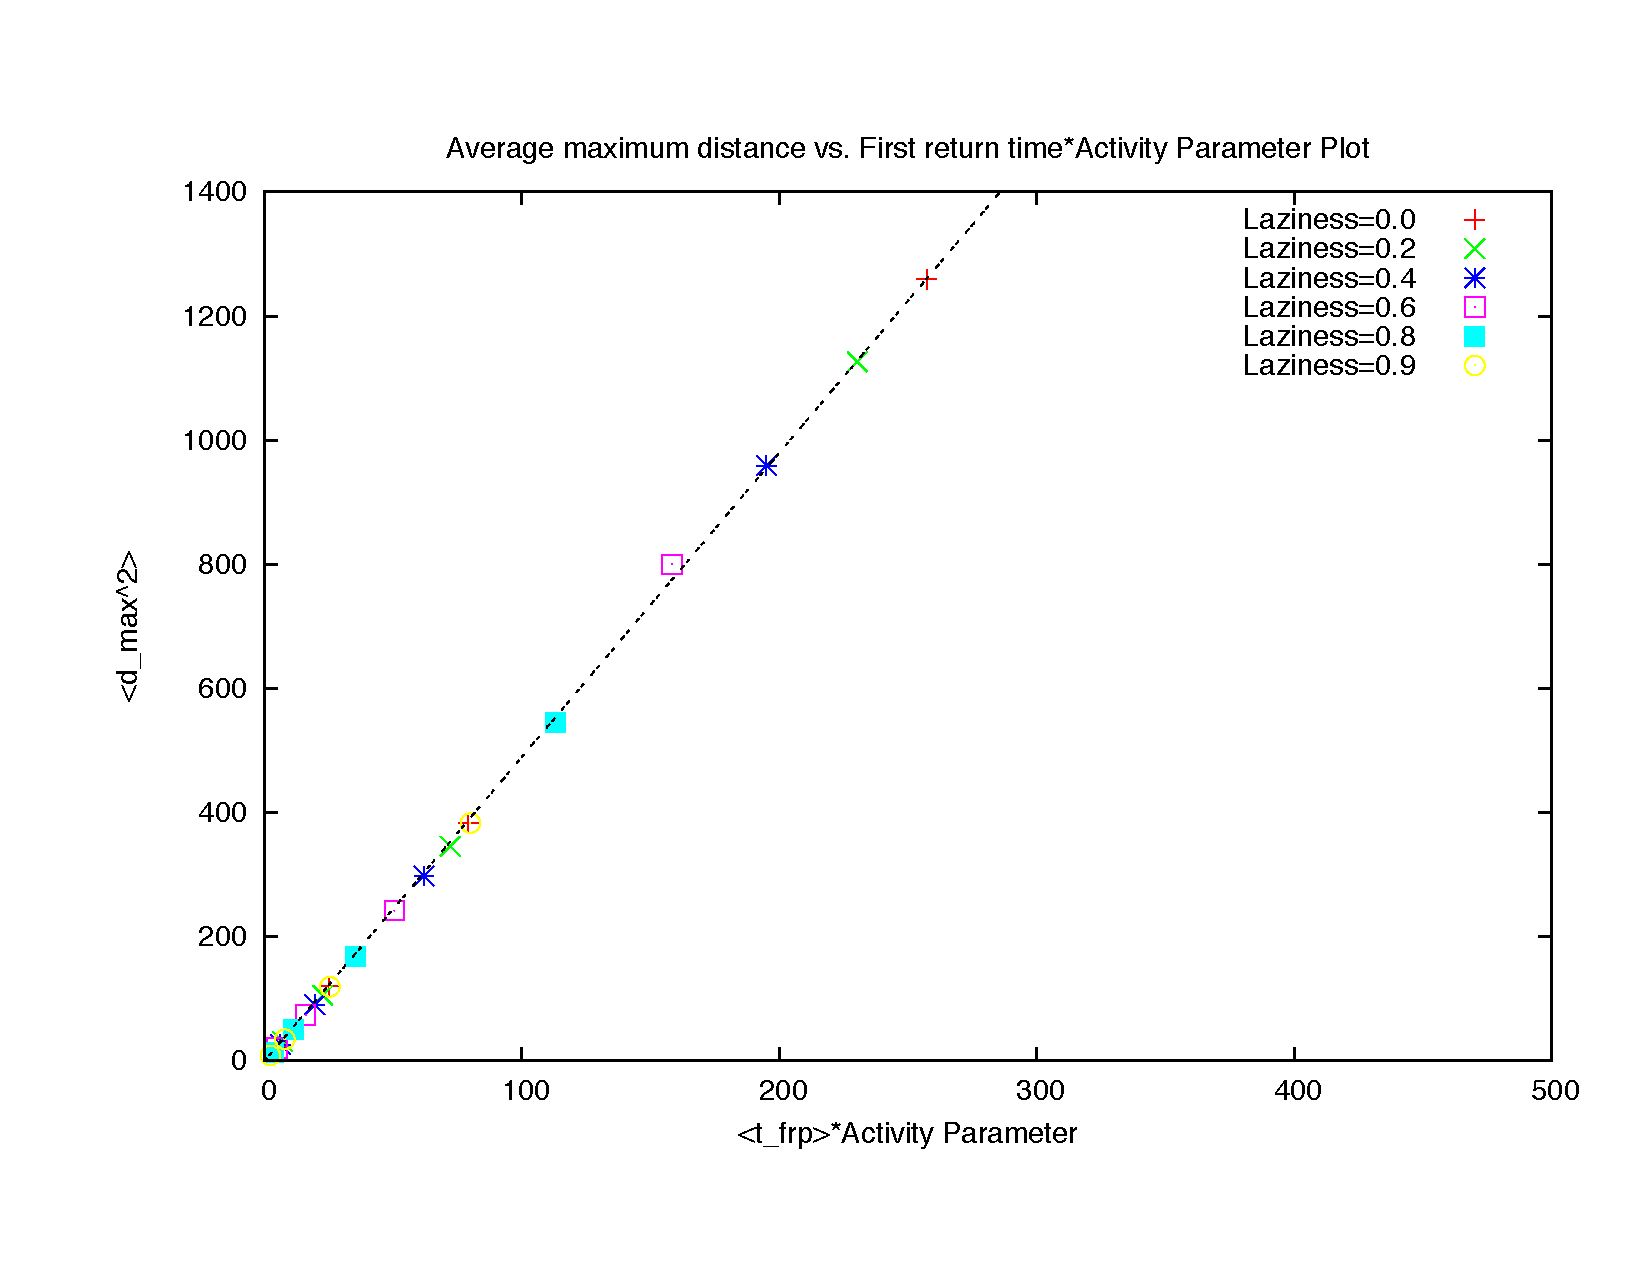
\includegraphics[width=\textwidth]{tfrp_scaled.pdf}
\caption{$\langle d_{{max}} \rangle ^2$ vs. $\langle t_{FR} \rangle\times P_{act}$ plot for laziness from 0 to 0.9, and $t_{max}$ ranging from 100 to 100000 in a geometric progression. Each $t_{max}$ has a group of points, and in each group the points are arranged in decreasing order of laziness.}
\label{fig:pow_law2}
\end{figure}
\end{document}
